\begin{figure}[!h]
	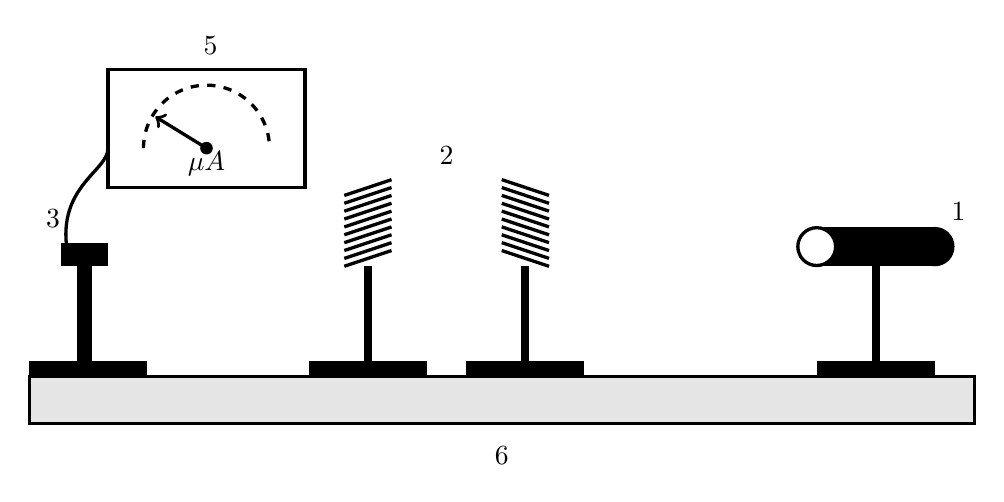
\begin{tikzpicture}[line width=1.2pt]
		
		%лава
		\fill[gray!20] (-6,0) rectangle (6,0.6);
		\draw (-6,0) rectangle (6,0.6);
		\node at (0,-0.4) {6};
		
		%ліхтар
		\fill[black] (4,0.6) rectangle (5.5,0.8);
		\fill[black] (4.7,0.8) rectangle (4.8,2);
		\fill[black] (4,2) rectangle (5.5,2.5);
		\fill[black] (5.5,2.25) circle (0.25);
		\fill[white] (4,2.25) circle (0.24); 
		\draw (4,2.25) circle (0.24); 
		\node at (5.8,2.7) {1};
		
		% поляризатори
		
		% перший пол.
		\fill[black] (-2.45,0.6) rectangle (-0.95,0.8);
		\fill[black] (-1.75,0.8) rectangle (-1.65,2);
		
		\foreach \y in {2,2.1,...,3}
		\draw (-2,\y) -- (-1.4,\y+0.2);
		
		% другий пол.
		\fill[black] (-0.45,0.6) rectangle (1.05,0.8);
		\fill[black] (0.25,0.8) rectangle (0.35,2);
		
		\foreach \y in {2,2.1,...,3}
		\draw (0,\y+0.2) -- (0.6,\y);
		\node at (-0.7,3.4) {2};
		
		%детектор
		\fill[black] (-6,0.6) rectangle (-4.5,0.8);
		\fill[black] (-5.4,0.8) rectangle (-5.2,2);
		\fill[black] (-5.6,2) rectangle (-5,2.3);
		\node at (-5.7,2.6) {3};
		
		%амперметр
		\draw (-5,3) rectangle (-2.5,4.5);
		\draw[dashed] (-4.55,3.5) arc[start angle=180,end angle=0,radius=0.8];
		\draw[->] (-3.75,3.5) -- (-4.4,3.9);
		\fill (-3.75,3.5) circle (0.08);
		
		\draw (-5.5,2.1) .. controls (-5.7,3) and (-5,3.2) .. (-5,3.5);
		\node at (-3.75,3.3) {$\mu A$};
		\node at (-3.7,4.8) {5};
	\end{tikzpicture}
	\caption{Експериментальна установка до 1 досліду}
\end{figure}